\chapter{Implementation}
\label{chap:implementation}
This has the description of how you actually went about implementing the project.  This should be focused on the interesting challenges and how those related to the project.

\todo{add more here}

\begin{figure}[h]  %t top, b bottom, p page | you can also use h to try to get the figure to appear at the current location
  \centering
  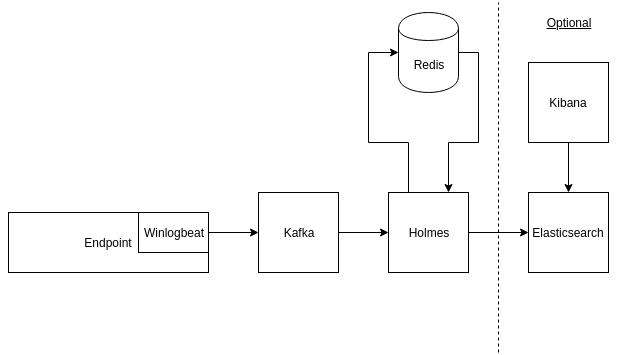
\includegraphics[width=.85\textwidth]{figures/holmes-architecture}
  \caption[An example figure.]{Minimal architecture. Every single node can be scaled both vertically and horizontally.}
  \label{fig:example}
\end{figure}